\documentclass{standalone}
\usepackage{pgfplots}
\usepackage{tikz}
\usepackage{xcolor}
\usetikzlibrary{arrows, decorations.pathmorphing}

\begin{document}
    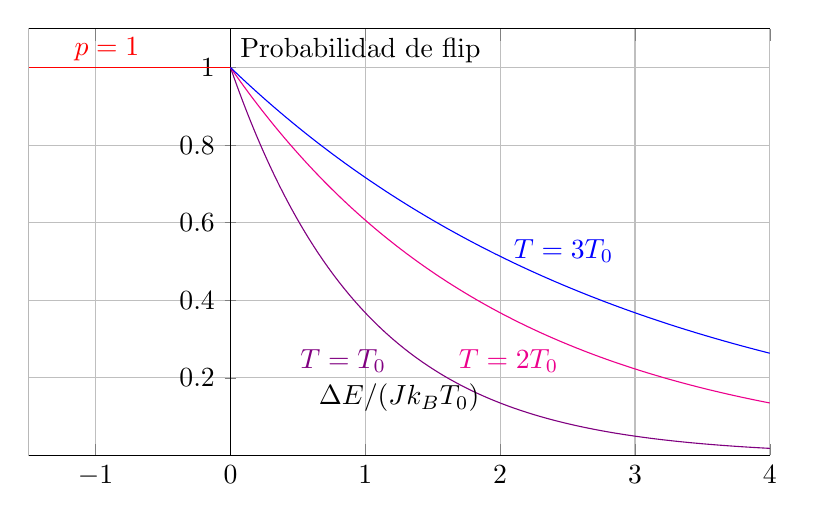
\begin{tikzpicture}[scale=1]
        \begin{axis}[width=110mm, height = 70mm,
            grid=both,
            xmin = -1.5, xmax = 4, ymin = 0, ymax = 1.1,
            axis y line=middle,
            x label style={at={(0.5,0.19)}},
            axis line style={-,color=black}, xlabel={$\Delta E/(Jk_{B}T_{0})$}, ylabel={Probabilidad de flip}] % 
            \addplot[domain=-1.5:0, restrict y to domain=0:3, samples=50, color=red ]{1};
            \addplot[domain=0:4, restrict y to domain=0:3,  samples=1000, color=violet ]{exp(-x)};
            \addplot[domain=0:4, restrict y to domain=0:3,  samples=1000, color=magenta ]{exp(-x/2)};
            \addplot[domain=0:4, restrict y to domain=0:3,  samples=1000, color=blue ]{exp(-x/3)};
        \end{axis}
        %\node[] at (2.0,0.4) {\textcolor{blue}{$p=e^{-\Delta E/(k_{B}T)}$}};
		\node[] at (1.0,5.16) {\textcolor{red}{$p=1$}};

        \node[] at (4.0,1.2) {\textcolor{violet}{$T=T_{0}$}};
        \node[] at (6.1,1.2) {\textcolor{magenta}{$T=2T_{0}$}};
        \node[] at (6.8,2.6) {\textcolor{blue}{$T=3T_{0}$}};

        \draw[color = black!28!white] (0,-0.0073) -- (0,5.426);
    \end{tikzpicture}
\end{document}